\clearpage

\subsection{Transparent with 1+1 Protection}\label{heuristic_Transp_Protection}
\begin{tcolorbox}	
\begin{tabular}{p{2.75cm} p{0.2cm} p{10.5cm}} 	
\textbf{Student Name}  &:& Pedro Coelho    (March 01, 2018 - )\\
\textbf{Goal}          &:& Implement the heuristic model for the transparent transport mode with 1 plus 1 protection.
\end{tabular}
\end{tcolorbox}

\subsubsection{Model description}

\vspace{11pt}
For this model, after the creation of the matrices and the network topology, it is necessary to apply the routing and grooming algorithms created. For the "Logical Topology" algorithm, the user must insert "Transparent" in the "logicalTopology" value and for the "Grooming" algorithm, the user must insert "no" in the parameter value "protection".

At the end, the "Cost Report" algorithm will be applied to obtain the best CAPEX result for the network in question.

We also must take into account the following particularity of this mode of transport:
\begin{itemize}
  \item $N_{OXC,n}$ = 1, \quad $\forall$ n that process traffic
  \item $N_{EXC,n}$ = 1, \quad $\forall$ n that process traffic
\end{itemize}

\vspace{11pt}
The minimization of the network CAPEX is made through the equation \ref{Capex_heuristic} where in this case for the cost of nodes we have in consideration the electric cost \ref{Capex_Node_EXC_heuristic} and the optical cost \ref{Capex_Node_OXC_heuristic}.
In this case the value of $P_{exc,c,n}$ is obtained by equation \ref{EXC_pexc_transparentp_heuristic_protec} and the value of $P_{oxc,n}$ is obtained by equation \ref{OXC_poxc_transparentp_heuristic_protec}.\\

The equation \ref{EXC_pexc_transparentp_heuristic_protec} refers to the number of short-reach ports of the electrical switch with bit-rate $c$ in node $n$, $P_{exc,c,n}$, i.e. the number of tributary ports with bit-rate $c$ in node $n$ which can be calculated as

\begin{equation}
P_{exc,c,n} = 2 \sum_{d=1}^{N} D_{nd,c}
\label{EXC_pexc_transparentp_heuristic_protec}
\end{equation}

\vspace{11pt}
where $D_{nd,c}$ are the client demands between nodes $n$ and $d$ with bit rate $c$.

\vspace{11pt}
In this case there is the following particularity:

\begin{itemize}
  \item When $n$=$d$ the value of client demands is always zero, i.e, $D_{nn,c}=0$
\end{itemize}

\vspace{11pt}
The equation \ref{OXC_poxc_transparentp_heuristic_protec} refers to the number of long-reach ports of the optical switch in node $n$, $P_{oxc,n}$, i.e. the number of line ports and the number of adding ports of node $n$ which can be calculated as

\begin{equation}
P_{oxc,n} = \sum_{j=1}^{N} f_{nj} + \sum_{j=1}^{N} \lambda_{nj}
\label{OXC_poxc_transparentp_heuristic_protec}
\end{equation}

\vspace{11pt}
where $f_{nj}$ refers to the number of line ports and $\lambda_{nj}$ refers to the number of adding ports.

\vspace{17pt}
The function, to be minimized, is the expression \ref{Minimize_Heuristic_CAPEX}.\\

\subsubsection{Result description}

It is already known all the necessary formulas to obtain the CAPEX value for the reference network \ref{Reference_Network_Topology}. As described in the subsection of the network traffic \ref{Reference_Network_Traffic}, it is necessary to obtain three different values of CAPEX for the low (0.5 Tbit/s), medium (5 Tbit/s) and high (10 Tbit/s) traffic. It is used a network software program called Net2Plan which can design the traffic matrices, create all the network topologies, simulate the algorithms into the network implemented in the programming software called Eclipse and analyze the results obtained.

In this chapter will be demonstrated the results by Vasco's heuristics from 2016. In each of the three traffic scenarios, it will be shown the network topologies followed by the table with the CAPEX value of the network.\\

\textbf{Low Traffic Scenario:}\\

In this scenario we have to take into account the traffic calculated in \ref{low_scenario}. In a first phase we will show the various existing topologies of the network. The first are the allowed topologies, physical and optical topology, the second are the logical topology for all ODUs and finally the resulting physical and optical topology.\\

\begin{figure}[H]
\centering
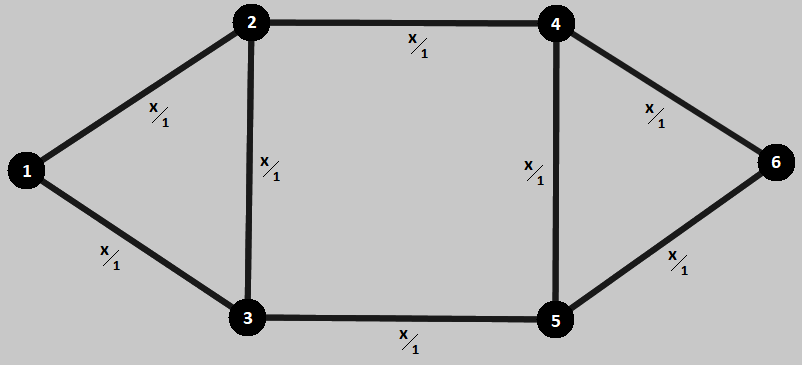
\includegraphics[width=13cm]{sdf/heuristic/transparent_protection/low/allowed_physical_low}
\caption{Allowed Physical Topology. The allowed physical topology is defined by the duct and sites in the field. It is assumed that each duct supports up to 1 bidirectional transmission system and each site supports up to 1 node.}
\label{allowed_physical_protection_ref_low_heuristic_transparent}
\end{figure}

\begin{figure}[H]
\centering
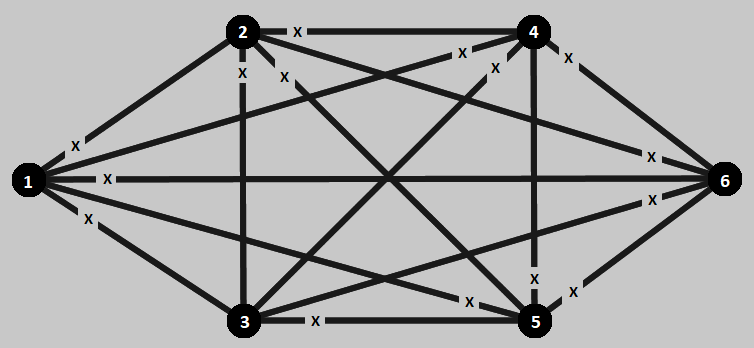
\includegraphics[width=13cm]{sdf/heuristic/transparent_protection/low/allowed_optical_low}
\caption{Allowed Optical Topology. The allowed optical topology is defined by the transport mode (transparent transport mode in this case). It is assumed that each connections between demands supports up to 100 lightpaths.}
\label{allowed_optical_protection_ref_low_heuristic_transparent}
\end{figure}

\begin{figure}[H]
\centering
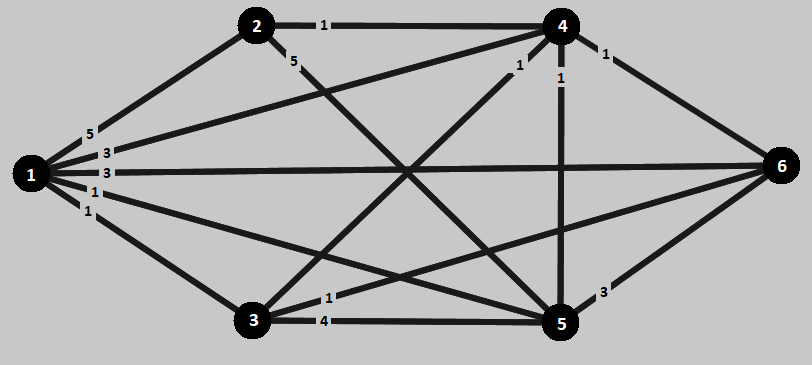
\includegraphics[width=13cm]{sdf/heuristic/transparent_protection/low/logical_topology_odu0_low}
\caption{ODU0 Logical Topology defined by the ODU0 traffic matrix.}
\label{logical_ODU0_protection_ref_low_heuristic_transparent}
\end{figure}

\begin{figure}[H]
\centering
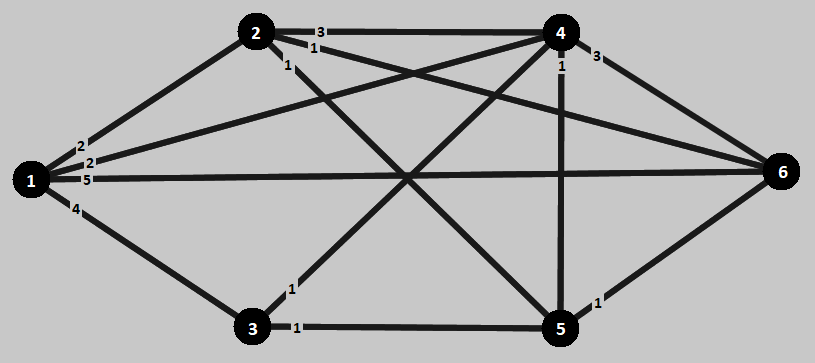
\includegraphics[width=13cm]{sdf/heuristic/transparent_protection/low/logical_topology_odu1_low}
\caption{ODU1 Logical Topology defined by the ODU1 traffic matrix.}
\label{logical_ODU1_protection_ref_low_heuristic_transparent}
\end{figure}

\begin{figure}[H]
\centering
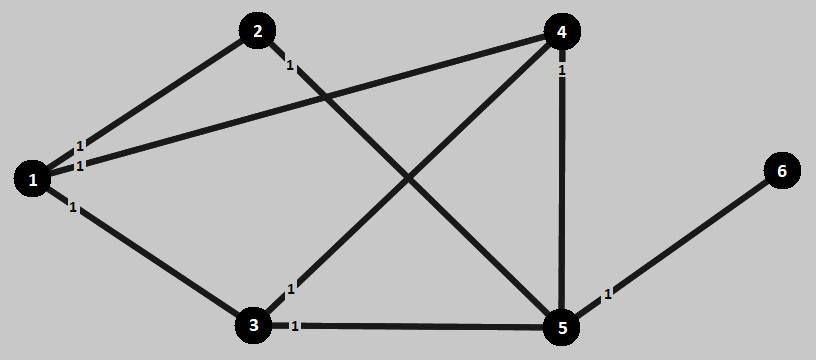
\includegraphics[width=13cm]{sdf/heuristic/transparent_protection/low/logical_topology_odu2_low}
\caption{ODU2 Logical Topology defined by the ODU2 traffic matrix.}
\label{logical_ODU2_protection_ref_low_heuristic_transparent}
\end{figure}

\begin{figure}[H]
\centering
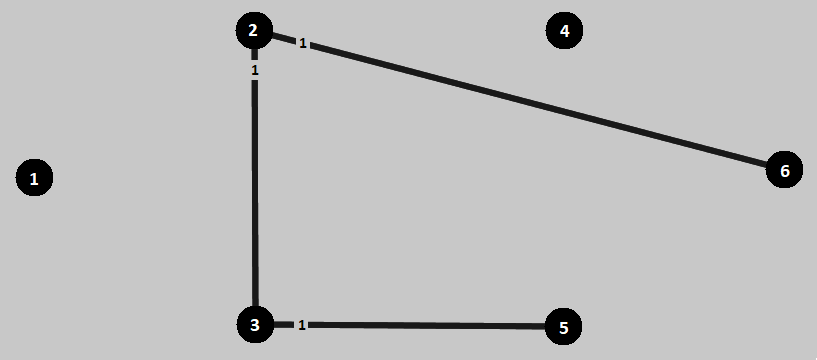
\includegraphics[width=13cm]{sdf/heuristic/transparent_protection/low/logical_topology_odu3_low}
\caption{ODU3 Logical Topology defined by the ODU3 traffic matrix.}
\label{logical_ODU3_protection_ref_low_heuristic_transparent}
\end{figure}

\begin{figure}[H]
\centering
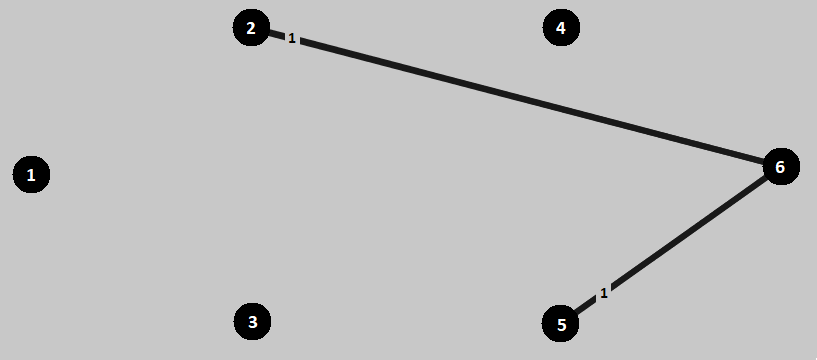
\includegraphics[width=13cm]{sdf/heuristic/transparent_protection/low/logical_topology_odu4_low}
\caption{ODU4 Logical Topology defined by the ODU4 traffic matrix.}
\label{logical_ODU4_protection_ref_low_heuristic_transparent}
\end{figure}

\begin{figure}[H]
\centering
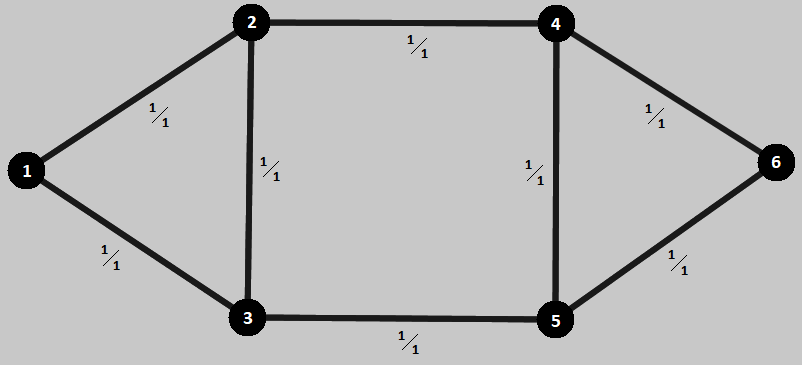
\includegraphics[width=13cm]{sdf/heuristic/transparent_protection/low/physical_topology_low}
\caption{Physical Topology after dimensioning.}
\label{physical_topology_protection_ref_low_heuristic_transparent}
\end{figure}

Following all the steps mentioned in the \ref{net2plan_guide}, applying the routing and grooming heuristic algorithms in the Net2Plan software and using all the data referring to this scenario, the obtained result for the Vasco's heuristics can be consulted in the following table \ref{scripttransp_protec_ref_low_heuristic}.

\begin{table}[H]
\centering
\begin{tabular}{|| c | c | c | c | c | c | c ||}
 \hline
 \multicolumn{7}{|| c ||}{CAPEX of the Network} \\
 \hline
 \hline
 \multicolumn{3}{|| c |}{ } & Quantity & Unit Price & Cost & Total \\
 \hline
 \multirow{3}{*}{Link Cost} & \multicolumn{2}{ c |}{OLTs} & 16 & 15 000 \euro & 240 000 \euro & \multirow{3}{*}{68 520 000 \euro} \\ \cline{2-6}
 & \multicolumn{2}{ c |}{100 Gb/s Transceivers} & 136 & 5 000 \euro/Gb/s & 68 000 000 \euro & \\ \cline{2-6}
 & \multicolumn{2}{ c |}{Amplifiers} & 70 & 4 000 \euro & 280 000 \euro & \\
 \hline
 \multirow{10}{*}{Node Cost} & \multirow{7}{*}{Electrical} & EXCs & 6 & 10 000 \euro & 60 000 \euro & \multirow{10}{*}{14 547 590 \euro} \\ \cline{3-6}
  & & ODU0 Ports & 60 & 10 \euro & 600 \euro & \\ \cline{3-6}
 & & ODU1 Ports & 50 & 15 \euro & 750 \euro & \\ \cline{3-6}
 & & ODU2 Ports & 16 & 30 \euro & 480 \euro & \\ \cline{3-6}
 & & ODU3 Ports & 6 & 60 \euro & 360 \euro & \\ \cline{3-6}
 & & ODU4 Ports & 4 & 100 \euro & 400 \euro & \\ \cline{3-6}
 & & Line Ports & 136 & 1 000 \euro/Gb/s & 13 600 000 \euro & \\ \cline{3-6}
 & \multirow{3}{*}{Optical} & OXCs & 6 & 20 000 \euro & 120 000 \euro & \\ \cline{3-6}
 & & Line Ports & 272 & 2 500 \euro/porto & 680 000 \euro & \\ \cline{3-6}
 & & Add Ports & 34 & 2 500 \euro/porto & 85 000 \euro & \\
 \hline
 \multicolumn{6}{|| c |}{Total Network Cost} & 83 067 590 \euro \\
\hline
\end{tabular}
\caption{Table with detailed description of CAPEX of Vasco's 2016 results.}
\label{scripttransp_protec_ref_low_heuristic}
\end{table}

\textbf{Medium Traffic Scenario:}\\

In this scenario we have to take into account the traffic calculated in \ref{medium_traffic_scenario}. In a first phase we will show the various existing topologies of the network. The first are the allowed topologies, physical and optical topology, the second are the logical topology for all ODUs and finally the resulting physical and optical topology.\\

\begin{figure}[H]
\centering
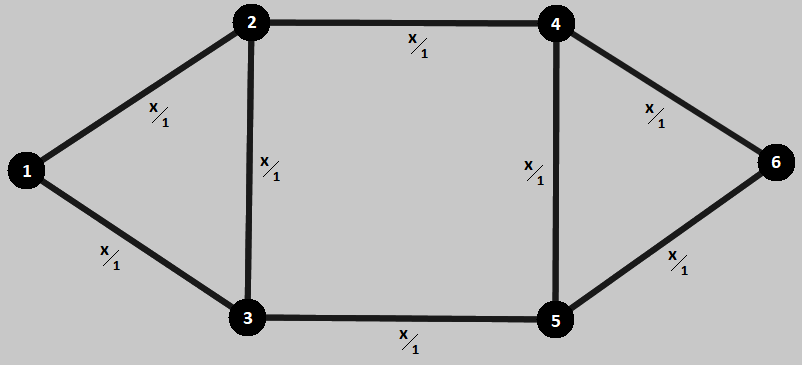
\includegraphics[width=13cm]{sdf/heuristic/transparent_protection/medium/allowed_physical_medium}
\caption{Allowed Physical Topology. The allowed physical topology is defined by the duct and sites in the field. It is assumed that each duct supports up to 1 bidirectional transmission system and each site supports up to 1 node.}
\label{allowed_physical_protection_ref_medium_heuristic_transparent}
\end{figure}

\begin{figure}[H]
\centering
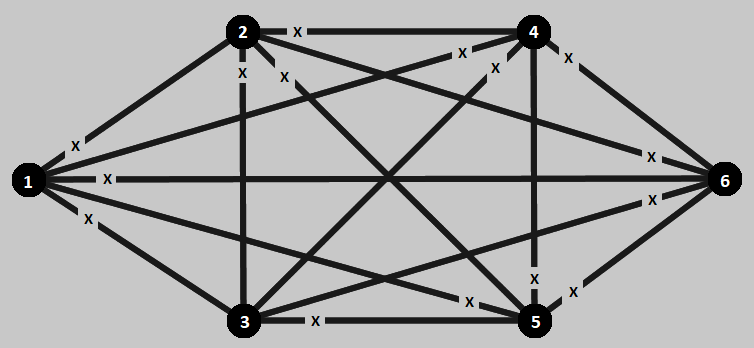
\includegraphics[width=13cm]{sdf/heuristic/transparent_protection/medium/allowed_optical_medium}
\caption{Allowed Optical Topology. The allowed optical topology is defined by the transport mode (transparent transport mode in this case). It is assumed that each connections between demands supports up to 100 lightpaths.}
\label{allowed_optical_protection_ref_medium_heuristic_transparent}
\end{figure}

\begin{figure}[H]
\centering
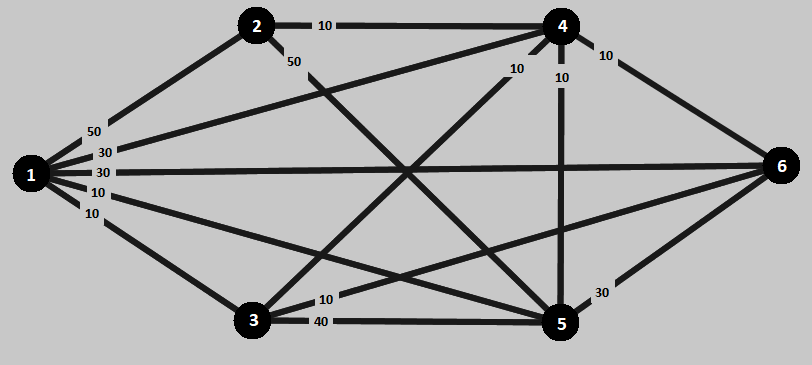
\includegraphics[width=13cm]{sdf/heuristic/transparent_protection/medium/logical_topology_odu0_medium}
\caption{ODU0 Logical Topology defined by the ODU0 traffic matrix.}
\label{logical_ODU0_protection_ref_medium_heuristic_transparent}
\end{figure}

\begin{figure}[H]
\centering
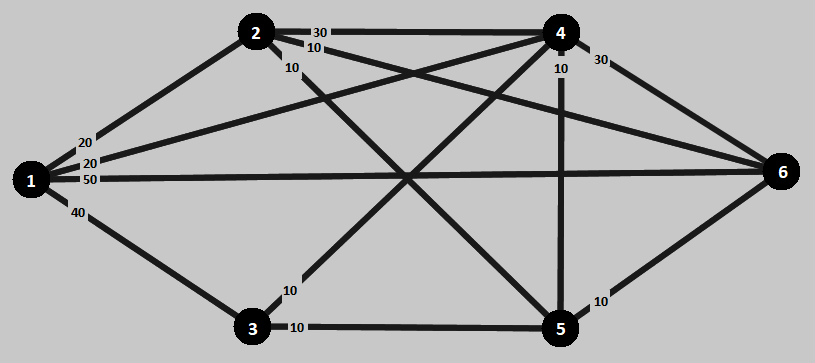
\includegraphics[width=13cm]{sdf/heuristic/transparent_protection/medium/logical_topology_odu1_medium}
\caption{ODU1 Logical Topology defined by the ODU1 traffic matrix.}
\label{logical_ODU1_protection_ref_medium_heuristic_transparent}
\end{figure}

\begin{figure}[H]
\centering
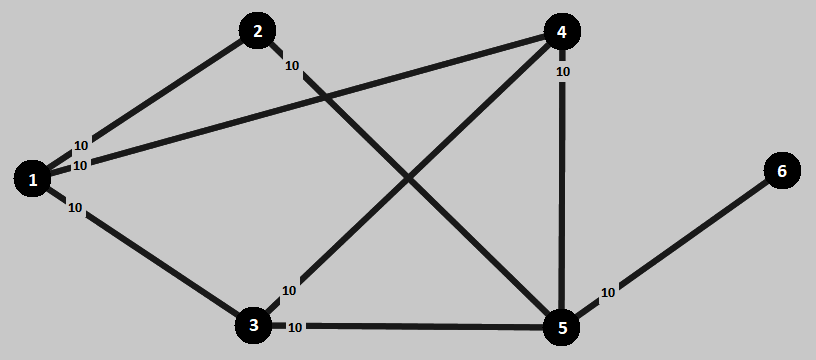
\includegraphics[width=13cm]{sdf/heuristic/transparent_protection/medium/logical_topology_odu2_medium}
\caption{ODU2 Logical Topology defined by the ODU2 traffic matrix.}
\label{logical_ODU2_protection_ref_medium_heuristic_transparent}
\end{figure}

\begin{figure}[H]
\centering
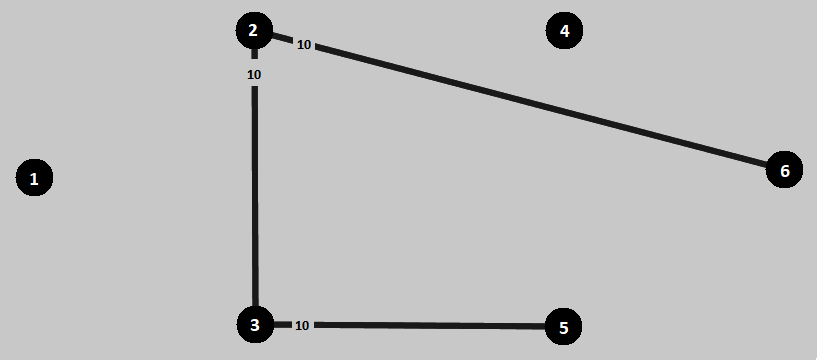
\includegraphics[width=13cm]{sdf/heuristic/transparent_protection/medium/logical_topology_odu3_medium}
\caption{ODU3 Logical Topology defined by the ODU3 traffic matrix.}
\label{logical_ODU3_protection_ref_medium_heuristic_transparent}
\end{figure}

\begin{figure}[H]
\centering
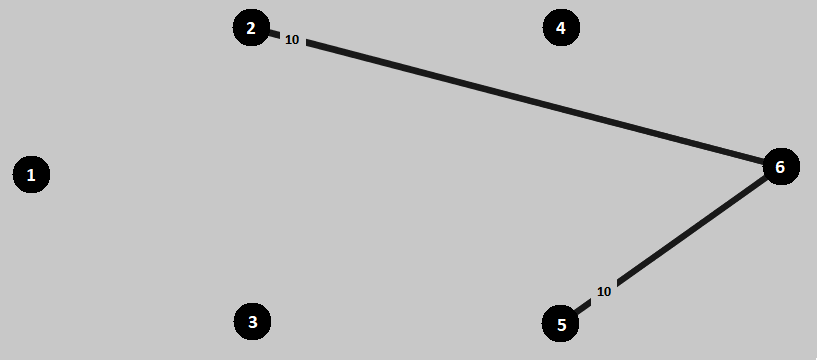
\includegraphics[width=13cm]{sdf/heuristic/transparent_protection/medium/logical_topology_odu4_medium}
\caption{ODU4 Logical Topology defined by the ODU4 traffic matrix.}
\label{logical_ODU4_protection_ref_medium_heuristic_transparent}
\end{figure}

\begin{figure}[H]
\centering
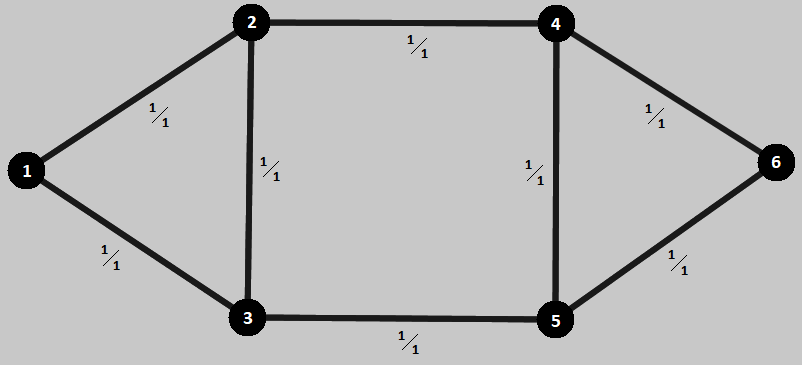
\includegraphics[width=13cm]{sdf/heuristic/transparent_protection/medium/physical_topology_medium}
\caption{Physical Topology after dimensioning.}
\label{physical_topology_protection_ref_medium_heuristic_transparent}
\end{figure}

Following all the steps mentioned in the \ref{net2plan_guide}, applying the routing and grooming heuristic algorithms in the Net2Plan software and using all the data referring to this scenario, the obtained result for the Vasco's heuristics can be consulted in the following table \ref{scripttransp_protec_ref_medium_heuristic}.

\begin{table}[H]
\centering
\begin{tabular}{|| c | c | c | c | c | c | c ||}
 \hline
 \multicolumn{7}{|| c ||}{CAPEX of the Network} \\
 \hline
 \hline
 \multicolumn{3}{|| c |}{ } & Quantity & Unit Price & Cost & Total \\
 \hline
 \multirow{3}{*}{Link Cost} & \multicolumn{2}{ c |}{OLTs} & 16 & 15 000 \euro & 240 000 \euro & \multirow{3}{*}{283 520 000 \euro} \\ \cline{2-6}
 & \multicolumn{2}{ c |}{100 Gb/s Transceivers} & 566 & 5 000 \euro/Gb/s & 283 000 000 \euro & \\ \cline{2-6}
 & \multicolumn{2}{ c |}{Amplifiers} & 70 & 4 000 \euro & 280 000 \euro & \\
 \hline
 \multirow{10}{*}{Node Cost} & \multirow{7}{*}{Electrical} & EXCs & 6 & 10 000 \euro & 60 000 \euro & \multirow{10}{*}{59 990 900 \euro} \\ \cline{3-6}
 & & ODU0 Ports & 600 & 10 \euro & 6 000 \euro & \\ \cline{3-6}
 & & ODU1 Ports & 500 & 15 \euro & 7 500 \euro & \\ \cline{3-6}
 & & ODU2 Ports & 160 & 30 \euro & 4 800 \euro & \\ \cline{3-6}
 & & ODU3 Ports & 60 & 60 \euro & 3 600 \euro & \\ \cline{3-6}
 & & ODU4 Ports & 40 & 100 \euro & 4 000 \euro & \\ \cline{3-6}
 & & Line Ports & 566 & 1 000 \euro/Gb/s & 56 600 000 \euro & \\ \cline{3-6}
 & \multirow{3}{*}{Optical} & OXCs & 6 & 20 000 \euro & 120 000 \euro & \\ \cline{3-6}
 & & Line Ports & 1 132 & 2 500 \euro/porto & 2 830 000 \euro & \\ \cline{3-6}
 & & Add Ports & 142 & 2 500 \euro/porto & 355 000 \euro & \\
 \hline
 \multicolumn{6}{|| c |}{Total Network Cost} & 343 510 900 \euro \\
\hline
\end{tabular}
\caption{Table with detailed description of CAPEX of Vasco's 2016 results.}
\label{scripttransp_protec_ref_medium_heuristic}
\end{table}

\textbf{High Traffic Scenario:}\\

In this scenario we have to take into account the traffic calculated in \ref{high_traffic_scenario}. In a first phase we will show the various existing topologies of the network. The first are the allowed topologies, physical and optical topology, the second are the logical topology for all ODUs and finally the resulting physical and optical topology.\\

\begin{figure}[H]
\centering
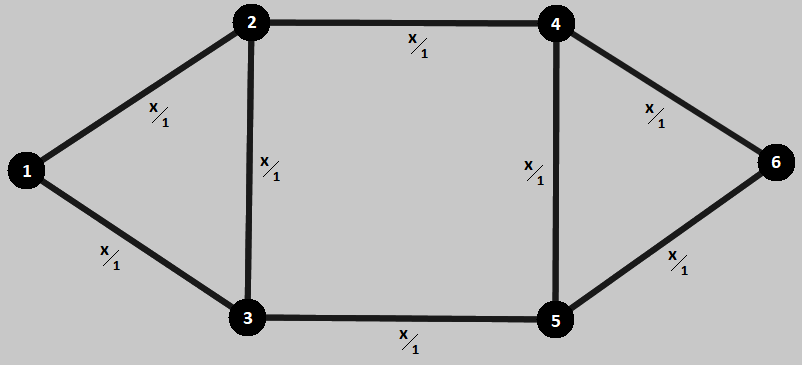
\includegraphics[width=13cm]{sdf/heuristic/transparent_protection/high/allowed_physical_high}
\caption{Allowed Physical Topology. The allowed physical topology is defined by the duct and sites in the field. It is assumed that each duct supports up to 1 bidirectional transmission system and each site supports up to 1 node.}
\label{allowed_physical_protection_ref_high_heuristic_transparent}
\end{figure}

\begin{figure}[H]
\centering
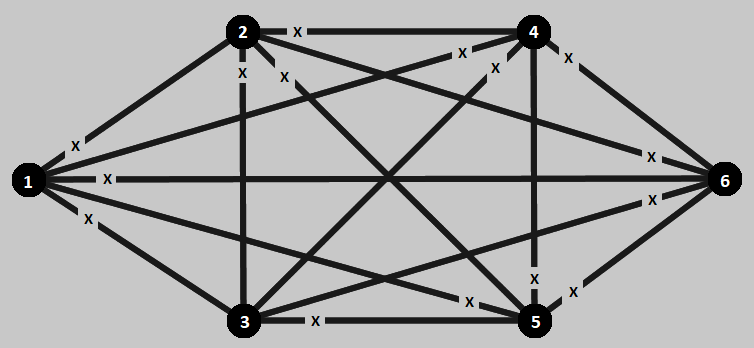
\includegraphics[width=13cm]{sdf/heuristic/transparent_protection/high/allowed_optical_high}
\caption{Allowed Optical Topology. The allowed optical topology is defined by the transport mode (transparent transport mode in this case). It is assumed that each connections between demands supports up to 100 lightpaths.}
\label{allowed_optical_protection_ref_high_heuristic_transparent}
\end{figure}

\begin{figure}[H]
\centering
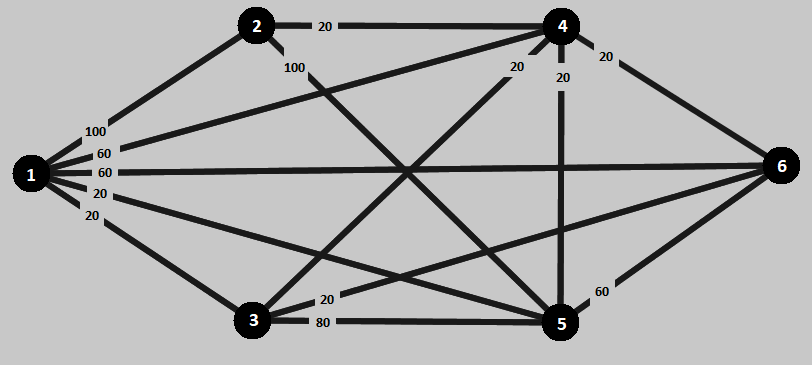
\includegraphics[width=13cm]{sdf/heuristic/transparent_protection/high/logical_topology_odu0_high}
\caption{ODU0 Logical Topology defined by the ODU0 traffic matrix.}
\label{logical_ODU0_protection_ref_high_heuristic_transparent}
\end{figure}

\begin{figure}[H]
\centering
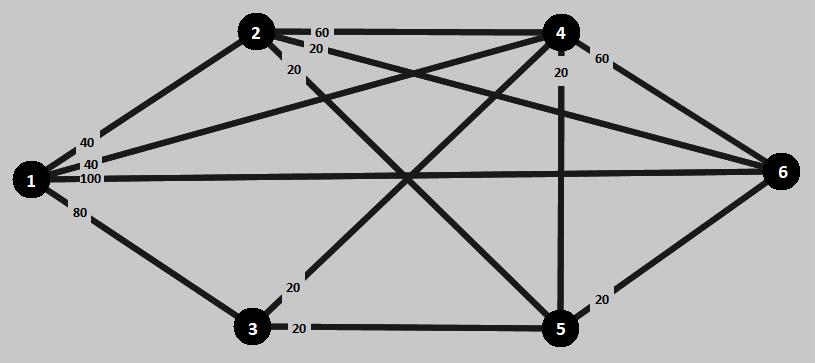
\includegraphics[width=13cm]{sdf/heuristic/transparent_protection/high/logical_topology_odu1_high}
\caption{ODU1 Logical Topology defined by the ODU1 traffic matrix.}
\label{logical_ODU1_protection_ref_high_heuristic_transparent}
\end{figure}

\begin{figure}[H]
\centering
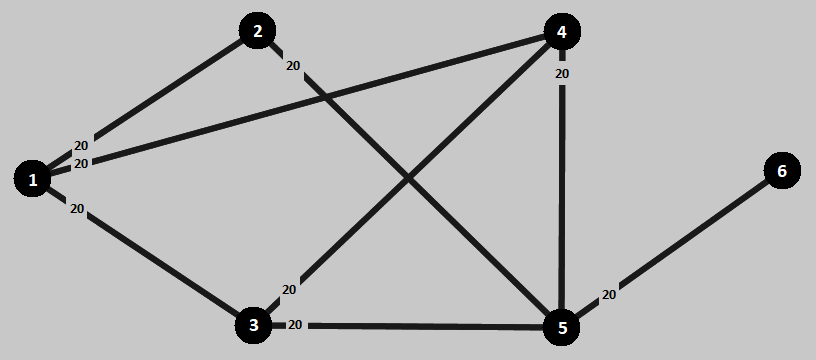
\includegraphics[width=13cm]{sdf/heuristic/transparent_protection/high/logical_topology_odu2_high}
\caption{ODU2 Logical Topology defined by the ODU2 traffic matrix.}
\label{logical_ODU2_protection_ref_high_heuristic_transparent}
\end{figure}

\begin{figure}[H]
\centering
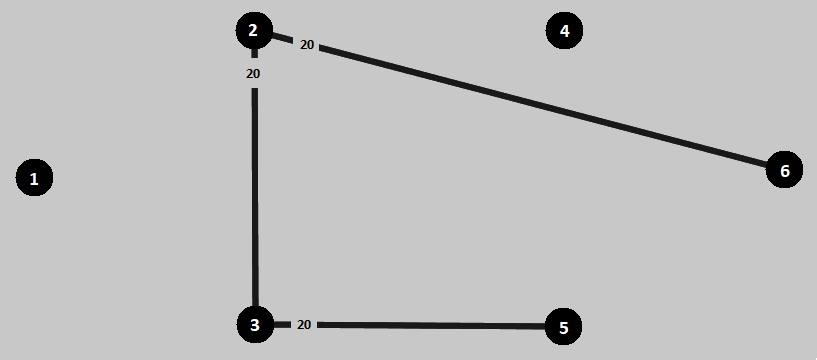
\includegraphics[width=13cm]{sdf/heuristic/transparent_protection/high/logical_topology_odu3_high}
\caption{ODU3 Logical Topology defined by the ODU3 traffic matrix.}
\label{logical_ODU3_protection_ref_high_heuristic_transparent}
\end{figure}

\begin{figure}[H]
\centering
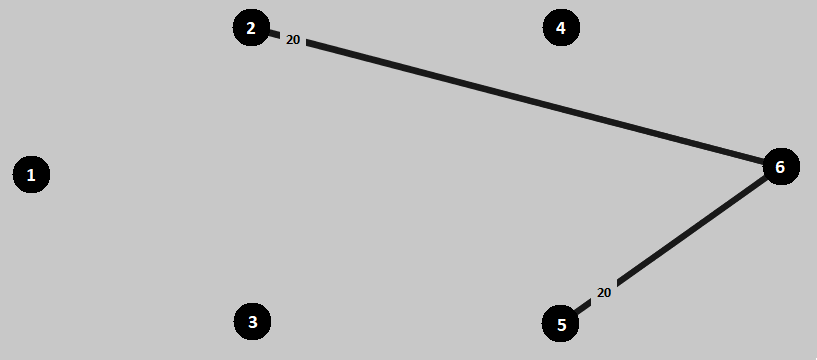
\includegraphics[width=13cm]{sdf/heuristic/transparent_protection/high/logical_topology_odu4_high}
\caption{ODU4 Logical Topology defined by the ODU4 traffic matrix.}
\label{logical_ODU4_protection_ref_high_heuristic_transparent}
\end{figure}

\begin{figure}[H]
\centering
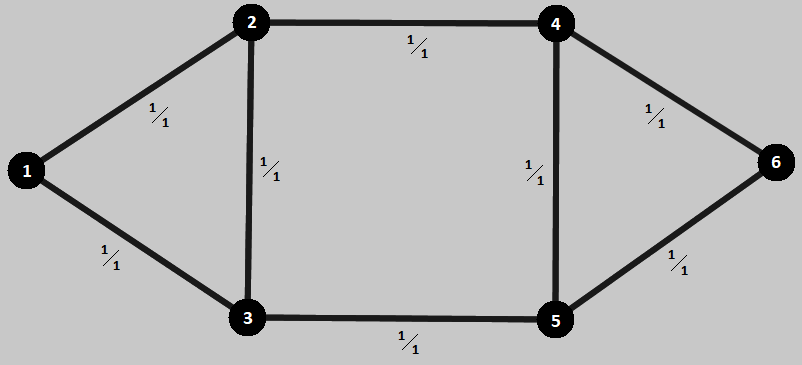
\includegraphics[width=13cm]{sdf/heuristic/transparent_protection/high/physical_topology_high}
\caption{Physical Topology after dimensioning.}
\label{physical_topology_protection_ref_high_heuristic_transparent}
\end{figure}

Following all the steps mentioned in the \ref{net2plan_guide}, applying the routing and grooming heuristic algorithms in the Net2Plan software and using all the data referring to this scenario, the obtained result for the Vasco's heuristics can be consulted in the following table \ref{scripttransp_protec_ref_high_heuristic}.

\begin{table}[H]
\centering
\begin{tabular}{|| c | c | c | c | c | c | c ||}
 \hline
 \multicolumn{7}{|| c ||}{CAPEX of the Network} \\
 \hline
 \hline
 \multicolumn{3}{|| c |}{ } & Quantity & Unit Price & Cost & Total \\
 \hline
 \multirow{3}{*}{Link Cost} & \multicolumn{2}{ c |}{OLTs} & 16 & 15 000 \euro & 240 000 \euro & \multirow{3}{*}{530 520 000 \euro} \\ \cline{2-6}
 & \multicolumn{2}{ c |}{100 Gb/s Transceivers} & 1 060 & 5 000 \euro/Gb/s & 530 000 000 \euro & \\ \cline{2-6}
 & \multicolumn{2}{ c |}{Amplifiers} & 70 & 4 000 \euro & 280 000 \euro & \\
 \hline
 \multirow{10}{*}{Node Cost} & \multirow{7}{*}{Electrical} & EXCs & 6 & 10 000 \euro & 60 000 \euro & \multirow{10}{*}{112 201 800 \euro} \\ \cline{3-6}
  & & ODU0 Ports & 1 200 & 10 \euro & 12 000 \euro & \\ \cline{3-6}
 & & ODU1 Ports & 1 000 & 15 \euro & 15 000 \euro & \\ \cline{3-6}
 & & ODU2 Ports & 320 & 30 \euro & 9 600 \euro & \\ \cline{3-6}
 & & ODU3 Ports & 120 & 60 \euro & 7 200 \euro & \\ \cline{3-6}
 & & ODU4 Ports & 80 & 100 \euro & 8 000 \euro & \\ \cline{3-6}
 & & Line Ports & 1 060 & 1 000 \euro/Gb/s & 106 000 000 \euro & \\ \cline{3-6}
 & \multirow{3}{*}{Optical} & OXCs & 6 & 20 000 \euro & 120 000 \euro & \\ \cline{3-6}
 & & Line Ports & 2 120 & 2 500 \euro/porto & 5 300 000 \euro & \\ \cline{3-6}
 & & Add Ports & 268 & 2 500 \euro/porto & 670 000 \euro & \\
 \hline
 \multicolumn{6}{|| c |}{Total Network Cost} & 642 721 800 \euro \\
\hline
\end{tabular}
\caption{Table with detailed description of CAPEX of Vasco's 2016 results.}
\label{scripttransp_protec_ref_high_heuristic}
\end{table}